% This file was created with matplot2tikz v0.5.4.
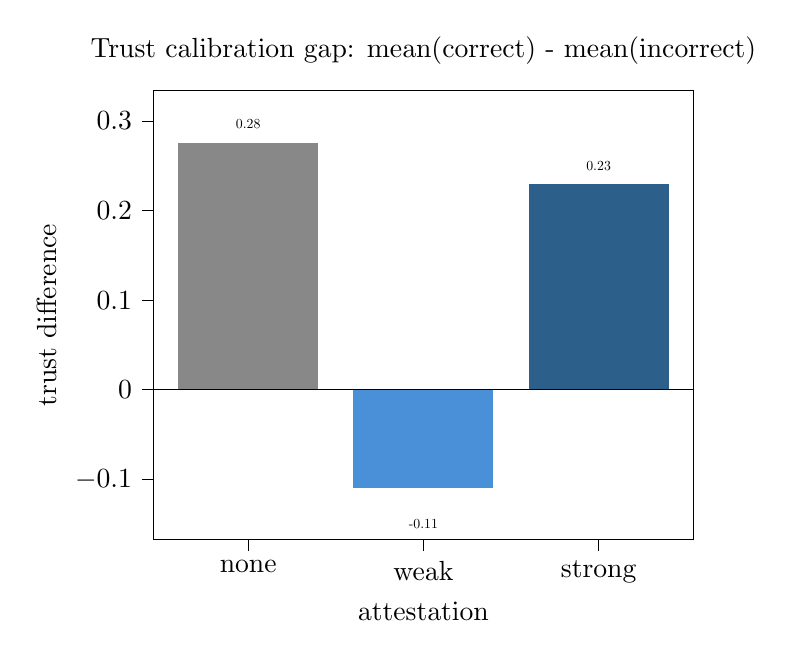
\begin{tikzpicture}

\definecolor{cornflowerblue74144217}{RGB}{74,144,217}
\definecolor{darkgray176}{RGB}{176,176,176}
\definecolor{darkslateblue4495138}{RGB}{44,95,138}
\definecolor{gray136}{RGB}{136,136,136}

\begin{axis}[
tick align=outside,
tick pos=left,
title={Trust calibration gap: mean(correct) - mean(incorrect)},
x grid style={darkgray176},
xlabel={attestation},
xmin=-0.54, xmax=2.54,
xtick style={color=black},
xtick={0,1,2},
xticklabels={none,weak,strong},
y grid style={darkgray176},
ylabel={trust difference},
ymin=-0.166954022988506, ymax=0.333620689655173,
ytick style={color=black}
]
\draw[draw=none,fill=gray136] (axis cs:-0.4,0) rectangle (axis cs:0.4,0.275862068965517);
\draw[draw=none,fill=cornflowerblue74144217] (axis cs:0.6,0) rectangle (axis cs:1.4,-0.109195402298851);
\draw[draw=none,fill=darkslateblue4495138] (axis cs:1.6,0) rectangle (axis cs:2.4,0.229885057471265);
\addplot [line width=0.32pt, black]
table {%
-0.54 0
2.54 0
};
\draw (axis cs:0,0.285862068965517) node[
  scale=0.5,
  anchor=south,
  text=black,
  rotate=0.0
]{0.28};
\draw (axis cs:1,-0.139195402298851) node[
  scale=0.5,
  anchor=north,
  text=black,
  rotate=0.0
]{-0.11};
\draw (axis cs:2,0.239885057471265) node[
  scale=0.5,
  anchor=south,
  text=black,
  rotate=0.0
]{0.23};
\end{axis}

\end{tikzpicture}
